\chapter{Versuchsaufbau}

\begin{figure}[H]
    \centering
    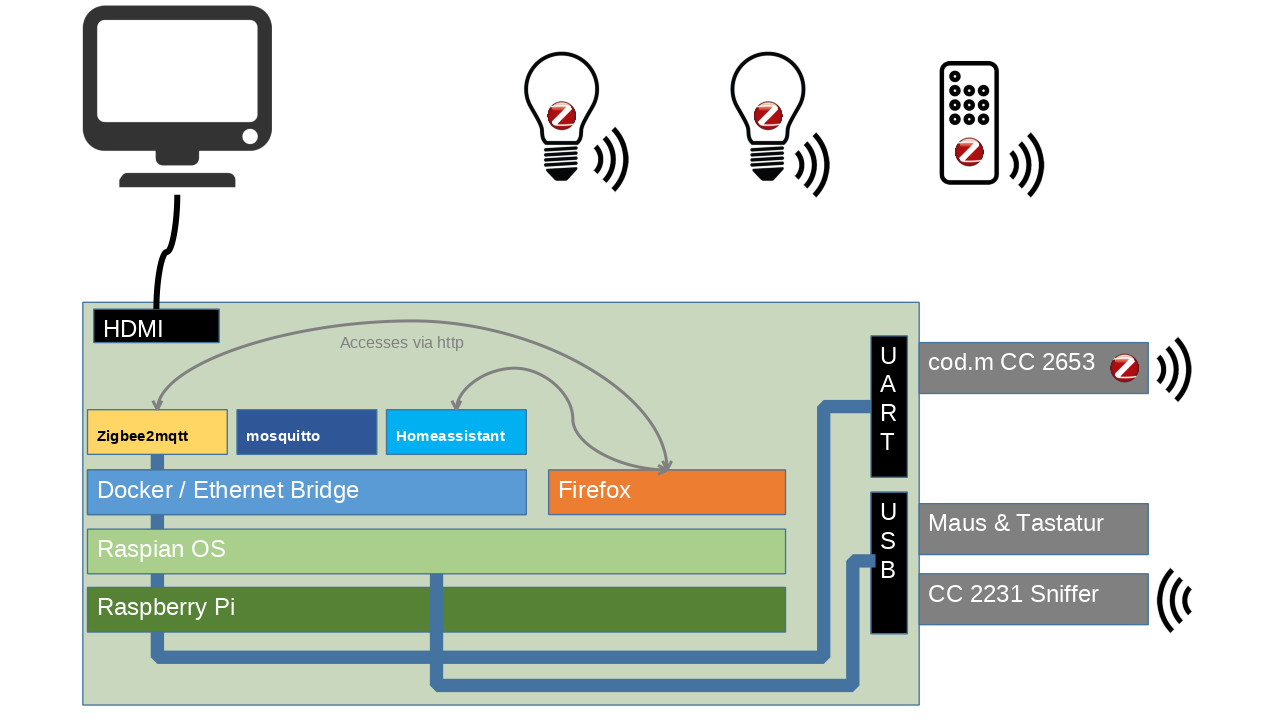
\includegraphics[width=1\textwidth]{media/Versuchsaufbau/image1.png}
    \caption{Versuchsaufbau}
  \end{figure}

In dieser Abbildung wird der schematische Versuchsaufbau gezeigt. Die drei Anwendungen werden als Docker Container gestartet. Sie kommunizieren
untereinander über eine eigenes Docker Netzwerk. Dies ist eine von Docker verwaltete Linux Bridge. Nur der NGINX Reverse Proxy hat zwei Ports, die
auf die Host Interface gemappt werden. Die Wegfrontends sind damit über den lokal installierten Browser erreichbar. Damit ist der Raspberry Applikationsserver
und Versuchs-PC zugleich.

Die Hostnames werden in der lokalen hosts Datei angelegt, damit die Namen Lokal ausfgelöst werden.

Der cod.m Zigbee Hat wird direkt an den Docker Container durchgereicht. Der Sniffer Stick ist regulär am Host angeschlossen. 